\documentclass[a5paper, 10pt]{article}
\usepackage[left=1cm, top=1.5cm, text={12.3cm, 16.8cm}]{geometry}
\usepackage[utf8x]{inputenc}
\usepackage[lf,default]{FiraSans}

% for graphics
\usepackage{picture}
\usepackage{graphicx}
\graphicspath{ {images/} }
\usepackage{listings}

% for maths
\usepackage{amsmath}
\usepackage{amsthm}
\usepackage{amssymb}

% for tabels
\usepackage[table]{xcolor}
\usepackage{enumitem}
\definecolor{gray}{HTML}{afafaf}
\usepackage{fontawesome5}
\usepackage{booktabs,makecell,xltabular}

\usepackage[os=win]{menukeys}
\renewmenumacro{\keys}[+]{shadowedroundedkeys}
\renewmenumacro{\menu}[>]{angularmenus}

\renewcommand{\tabularxcolumn}[1]{m{#1}}
\arrayrulecolor{gray}

% nifty commands by Paul Gaborit from http://tex.stackexchange.com/a/236891/226
\def\setmenukeyswin{\def\tw@mk@os{win}}

% others
\usepackage{hyperref}
\usepackage{textcomp}

\begin{document}

\begin{titlepage}
    \begin{center}
        \,\vspace{\stretch{0.25}}

        \Huge
        WaterLift Calculator\\

        \LARGE
        Version 1.0\\

        \vspace{\stretch{0.75}}
        \Large
        Team:               \hfill Blue Hair is the Way\\
        Last manual release:\hfill \today\\
        %Manual author: \hfill Evgenii Shiliaev
    \end{center}
\end{titlepage}

\tableofcontents
\pagebreak

\section{Important information}
    \emph{WaterLift Calculator} is a calculator application providing basic mathematical operations created for comfortable home counting.

    This application was developed as the second project of the \emph{"Practical Aspects of Software Design"} school subject by the team \emph{"Blue Hair is the Way"}

    \subsection{Supported platforms}
    \begin{table}[h]
        \vspace{-2em}
        \begin{xltabular}{\textwidth}{
            >{}l @{\hspace{2em}}
            >{\renewcommand\cellalign{cl}}X}
                 \textbf{Requirements}          & \textbf{Minimum}\\* \midrule
                 CPU                            & Any modern CPU\\* \midrule
                 Operating system               & 64-bit \faUbuntu Ubuntu 20.04 or newer\\* \midrule
        \end{xltabular}
        %\caption{Caption}
        \label{tab:Supported_platforms}
    \end{table}

    \subsection{Authors}
        "Blue Hair is the way" Team:
        \begin{itemize}
            \item Evgenii Shiliaev
            \item Marko Kubrachenko
            \item Pavel Beneš
            \item Šimon Brázda
        \end{itemize}

    \subsection{License}
        The project is licensed under the \href{https://choosealicense.com/licenses/gpl-3.0/}{GNU GPLv3} license.

\pagebreak

\section{Installation}
    \subsection{Via the installer}
        Download the last version installer of the application.
        \begin{itemize}
            \item Open the installer and click the \keys{Install} button
            \begin{figure}[h]
                \centering
                \scalebox{0.34}{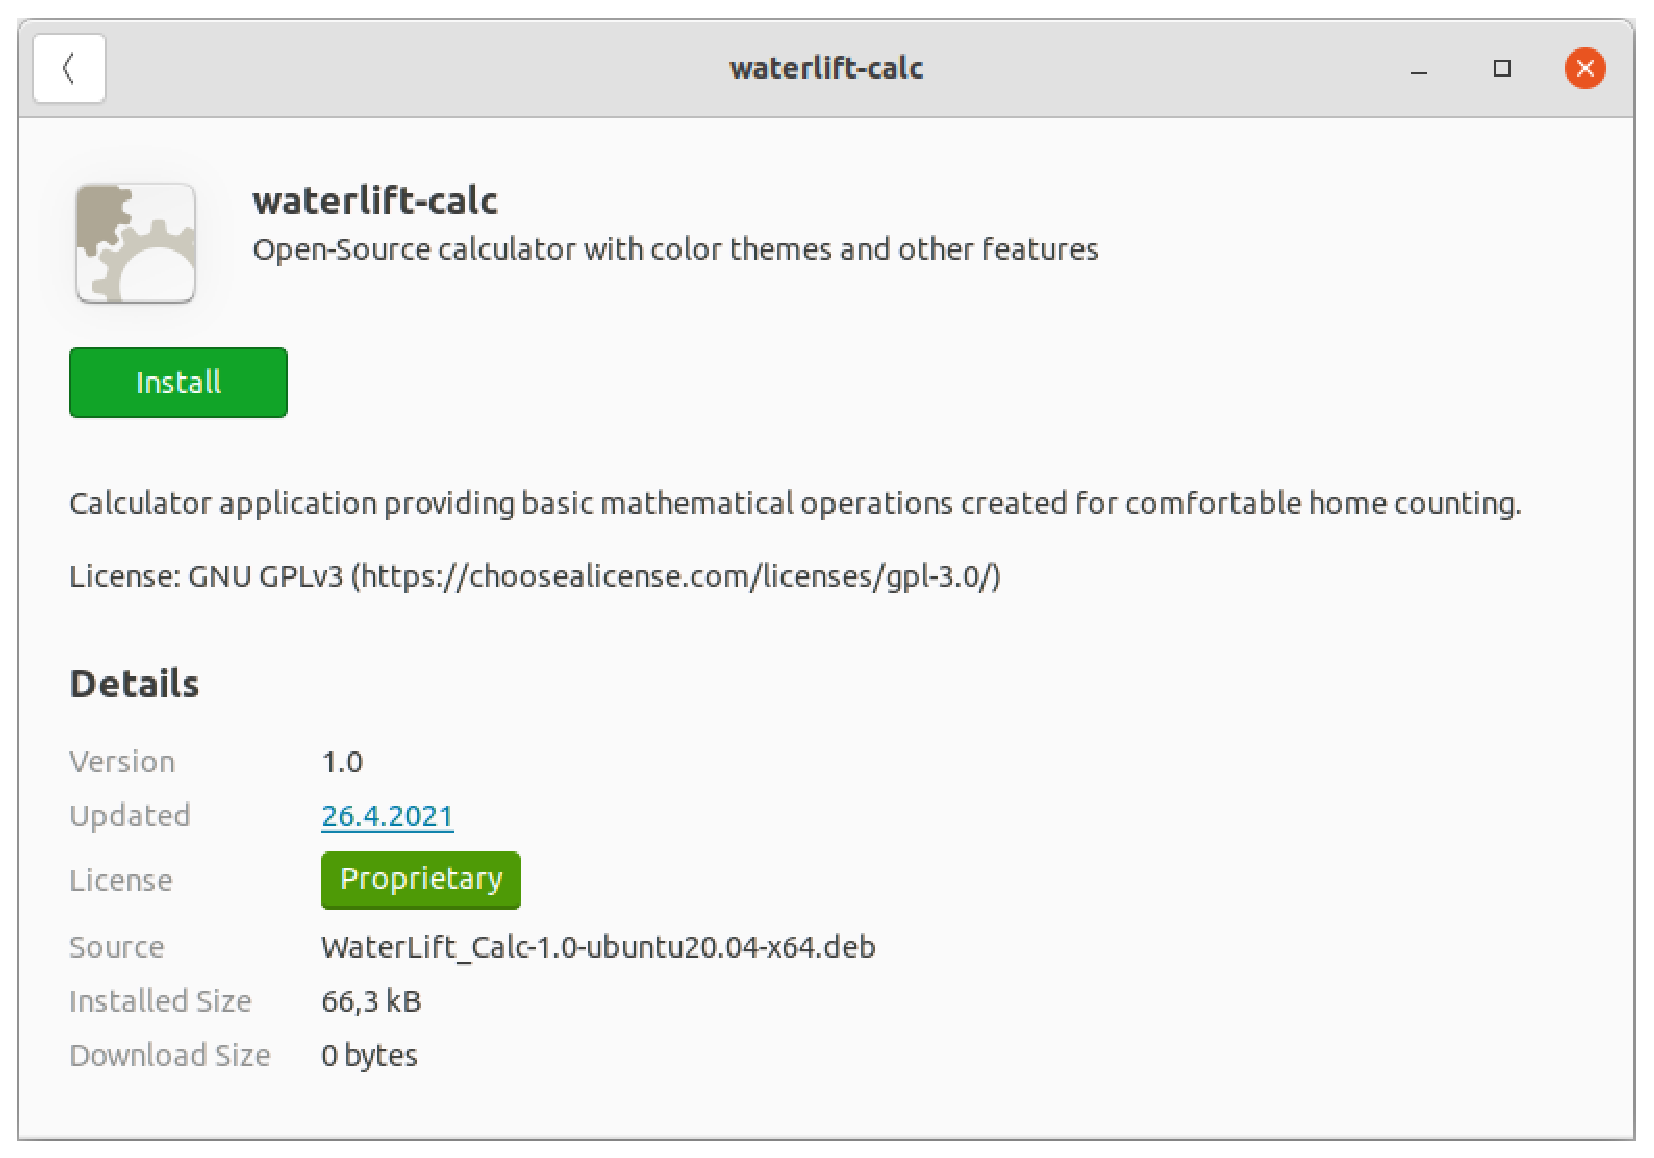
\includegraphics{installation.eps}}
                \caption{Installation window}
                \label{fig:installation_window}
            \end{figure}
    
            \item Or use CLI command:
            \lstset{language=bash, frame=lines}
            \begin{lstlisting}
sudo dpkg -i waterlift_calc-1.0-ubuntu20.04-x64.deb
            \end{lstlisting}
        \end{itemize}
        
    \subsection{Manually}
    Do all steps in the directory, where you have downloaded the necessary files.
    \begin{enumerate}
        \item Download source files and the icon:
            \begin{itemize}
                \item \texttt{gui.py}
                \item \texttt{math\_lib.py}
                \item \texttt{manual\_for\_hepl\_window.pdf}
        	    \item \texttt{waterlift\_calc\_logo.png}
            \end{itemize}
        \item Give yourself superuser rights
            \lstset{language=bash, frame=lines}
            \begin{lstlisting}
sudo -s
            \end{lstlisting}
        \item Make \texttt{gui.py} executable
        \lstset{language=bash, frame=lines}
            \begin{lstlisting}
chmod a+x gui.py
            \end{lstlisting}
        \item Change the path to the user manual in the gui.py by the following commands:
            \lstset{language=bash, frame=lines}
            \begin{lstlisting}
awk '{gsub("manual_for_help_window.pdf", "/usr/share/-
waterlift-calc/manual_for_help_window.pdf")}1' 
gui.py > tmp_gui.py

cat tmp_gui.py > gui.py
            \end{lstlisting}
            
        \item Change the path to the application icon in the gui.py by the following commands:
            \lstset{language=bash, frame=lines}
            \begin{lstlisting}
awk '{gsub("../images/waterlift_calc_logo.png","/usr/-
share/pixmaps/waterlift_calc_logo.png")}1' 
gui.py > tmp_gui.py 

cat tmp_gui.py > gui.py 

rm -f tmp_gui.py
            \end{lstlisting}
            
        \item Install the following packages:
            \begin{itemize}
                \item python3.8
	            \item python-tk
	            \item python3-pip
	            \item tkDocViewer
            \end{itemize}
            \lstset{language=bash, frame=lines}
            \begin{lstlisting}
apt-get install python3.8 python3-tk python3-pip

pip3 install tkDocViewer
            \end{lstlisting}
        \item Make a \texttt{waterlift\_calc} folder in \texttt{/usr/share/}
            \lstset{language=bash, frame=lines}
            \begin{lstlisting}
mkdir /usr/share/waterlift-calc
            \end{lstlisting}
        \item Copy to the \texttt{/usr/share/waterlift-calc} downloaded files (except the logo)
            \lstset{language=bash, frame=lines}
            \begin{lstlisting}
cp gui.py math_lib.py manual_for_help_window.pdf 
/usr/share/waterlift-calc
            \end{lstlisting}
        \item Copy to the \texttt{/usr/share/pixmaps} downloaded logo
            \lstset{language=bash, frame=lines}
            \begin{lstlisting}
cp waterlift_calc_logo.png /usr/share/pixmaps
            \end{lstlisting}
        \item Link the app to the system
            \lstset{language=bash, frame=lines}
            \begin{lstlisting}
ln -sf /usr/share/waterlift-calc/gui.py /usr/bin/-
waterlift-calc
            \end{lstlisting}
        \item In the \texttt{/usr/share/applications} make a \texttt{waterlift\_calc.desktop} file
        \lstset{language=bash, frame=lines}
            \begin{lstlisting}
nano /usr/share/applications/waterlift_calc.desktop
            \end{lstlisting}
        and write to it the followind text:
            \begin{lstlisting}
[Desktop Entry]
Version=1.0
Type=Application
Name=WaterLift Calculator
Comment=Basic mathematical operations color calculator
Exec=/usr/bin/waterlift-calc
Icon=/usr/share/pixmaps/waterlift_calc_logo.png
Categories=Utility
Terminal=false
StartupNotify=true
StartupWMClass=gui
Name[cs]=WaterLift Calculator
            \end{lstlisting}
    \end{enumerate}

\noindent
Now the app should appear in \emph{Show Applications}. If not, try to \textbf{log out} and \textbf{log in}.

\pagebreak

\section{Get started}
    \subsection{Run WaterLift Calculator}
        \begin{itemize}
            \item Go to the \emph{Show Applications} and click \emph{WaterLift Claculator}
            \begin{figure}[h]
                \centering
                \scalebox{0.34}{
\includegraphics{run_from_the_show_application.eps}}
                \caption{Run from the Show application}
                \label{fig:run_the_app}
            \end{figure}

            \item Or use CLI command:
            \lstset{language=bash, frame=lines}
            \begin{lstlisting}
waterlift-calc
            \end{lstlisting}
        \end{itemize}


    \subsection{Overview of the user interface}
        \begin{figure}[h]
            \centering
            \scalebox{0.65}{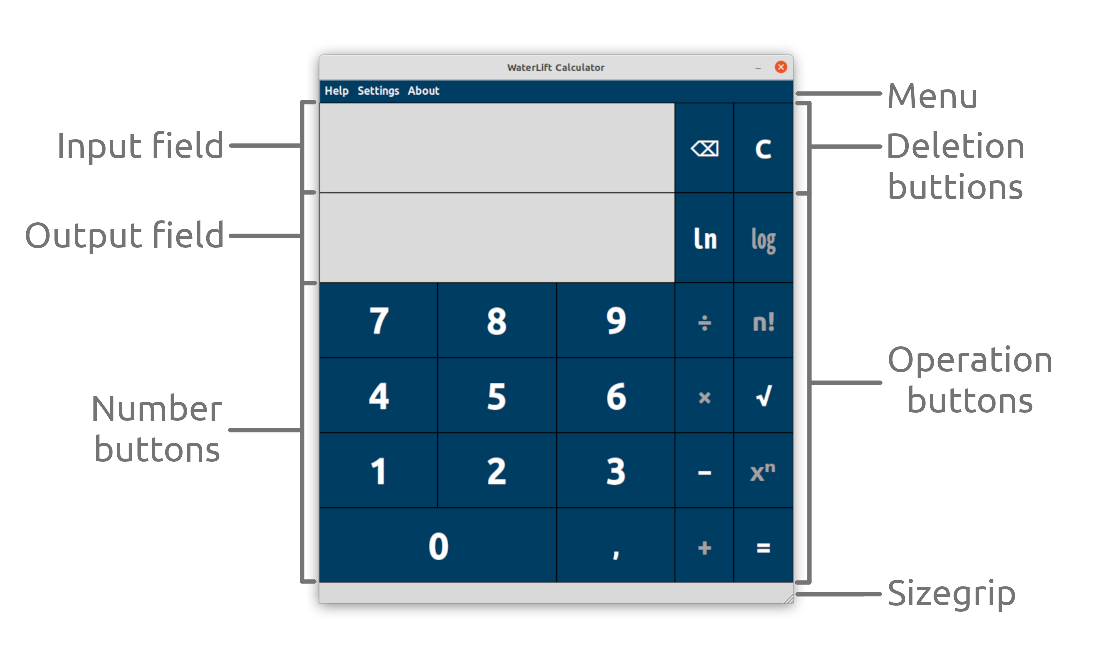
\includegraphics{user_interface01.eps}}
            \caption{Main window}
            \label{pic:UI_Main_Window_01}
        \end{figure}

    \subsection{Appearance}
        We also provide 7 color themes for your better calculating experience.
        \begin{figure}[h]
            \centering
            \scalebox{0.4}{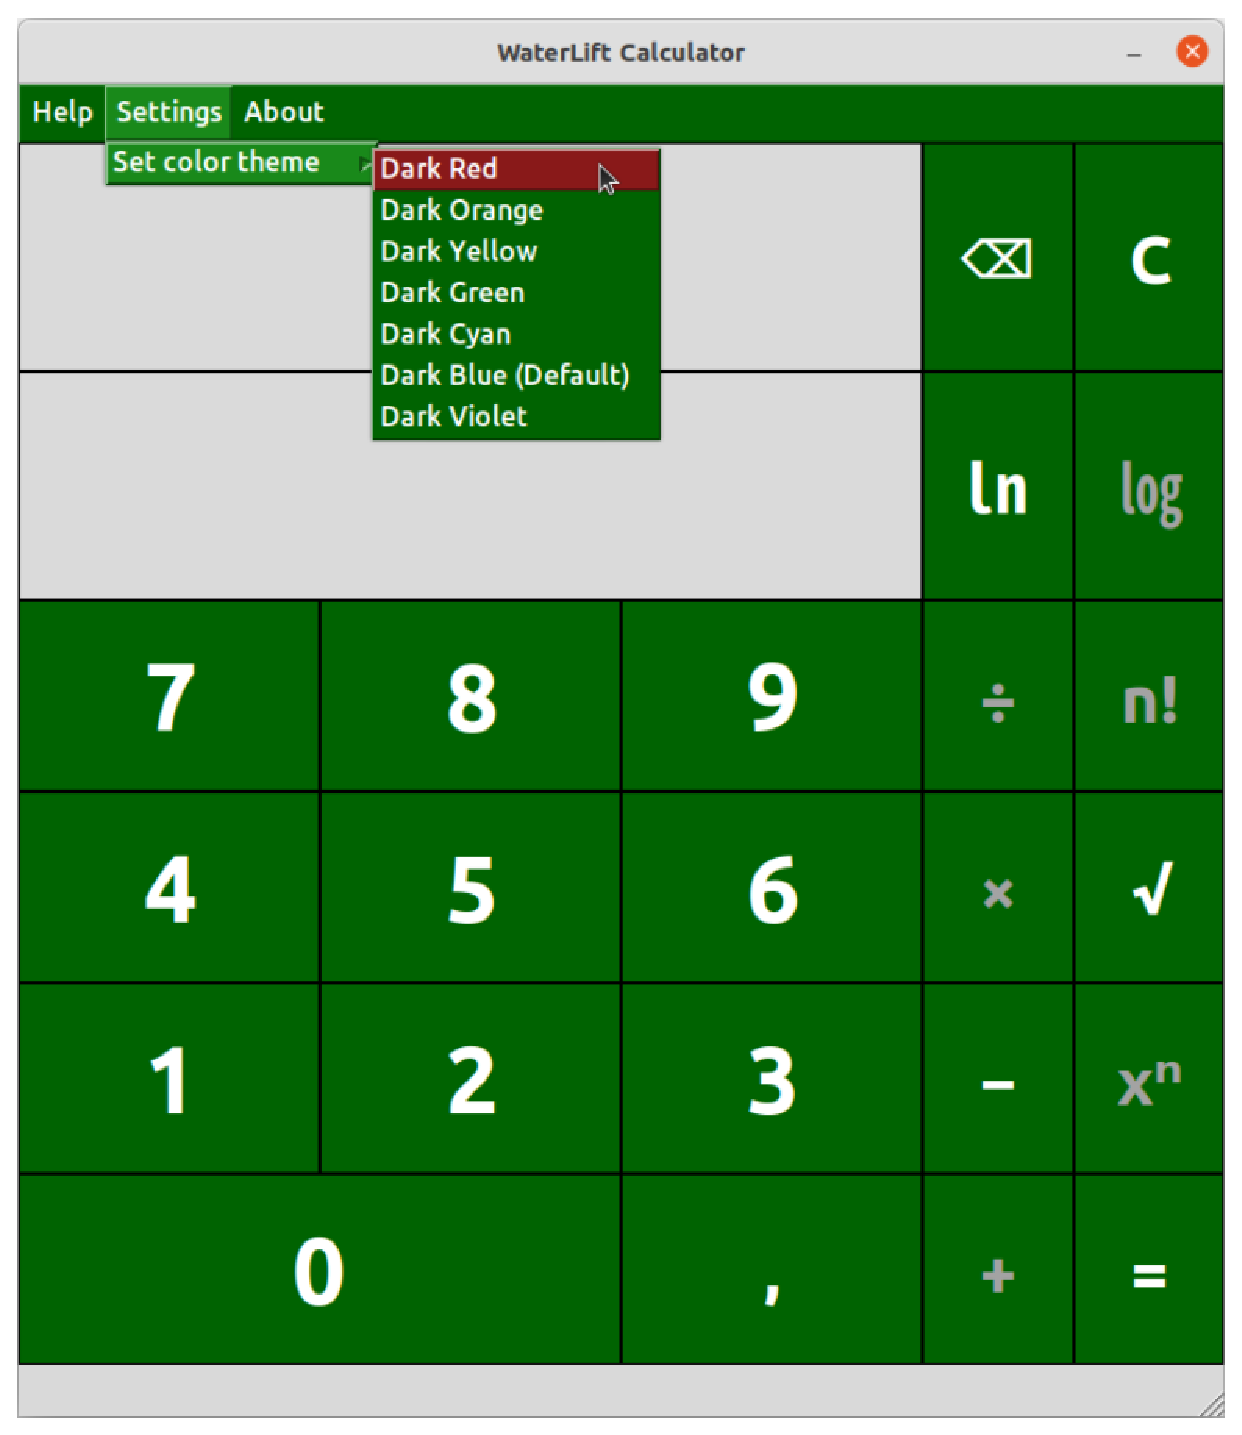
\includegraphics{user_interface02.eps}}
            \caption{Color scheme changing}
            \label{fig:UI_Main_Window_02}
        \end{figure}

    \subsection{Features}
        We have added some interesting features that can make your calculating much easier.
        \pagebreak
        \subsubsection{"No zero part"}
            No need to write zero in decimal numbers, the calculator add it by itself.
            \begin{figure}[h]
                \centering
                \scalebox{0.32}{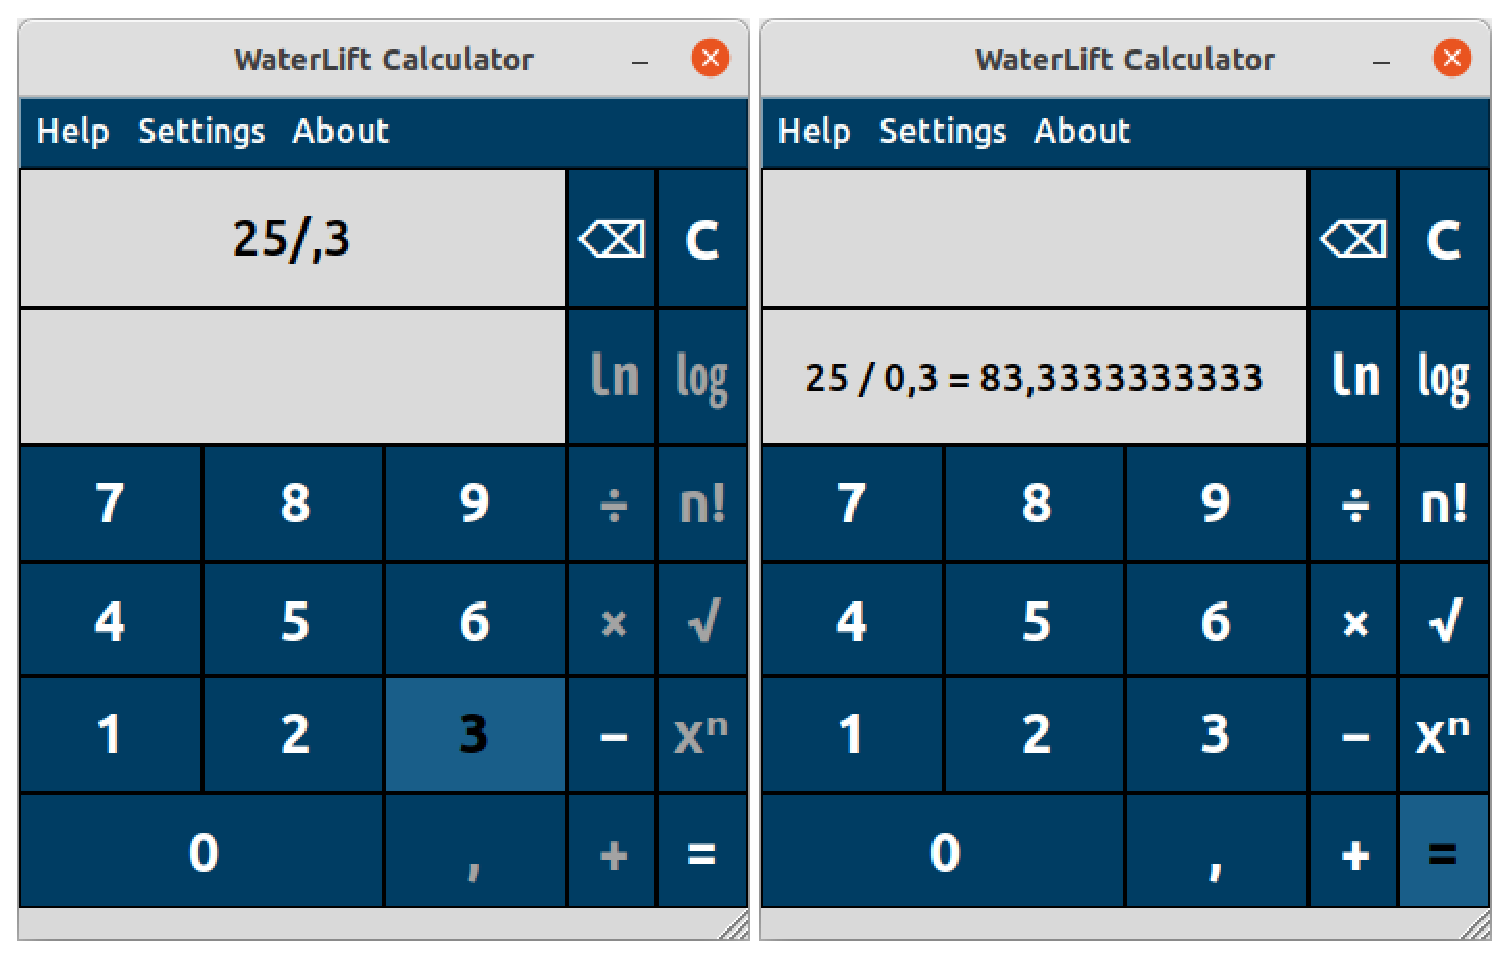
\includegraphics{no_zero_part.eps}}
                \caption{"No zero part" feature}
                \label{pic:"no_zero_part"}
            \end{figure}

        \subsubsection{"Continue the calculating"}
            After the evaluation of the last expression,
            \begin{itemize}
                \item press \keys{=} to put the result into the input field
                \begin{figure}[h]
                    \centering
                    \scalebox{0.32}{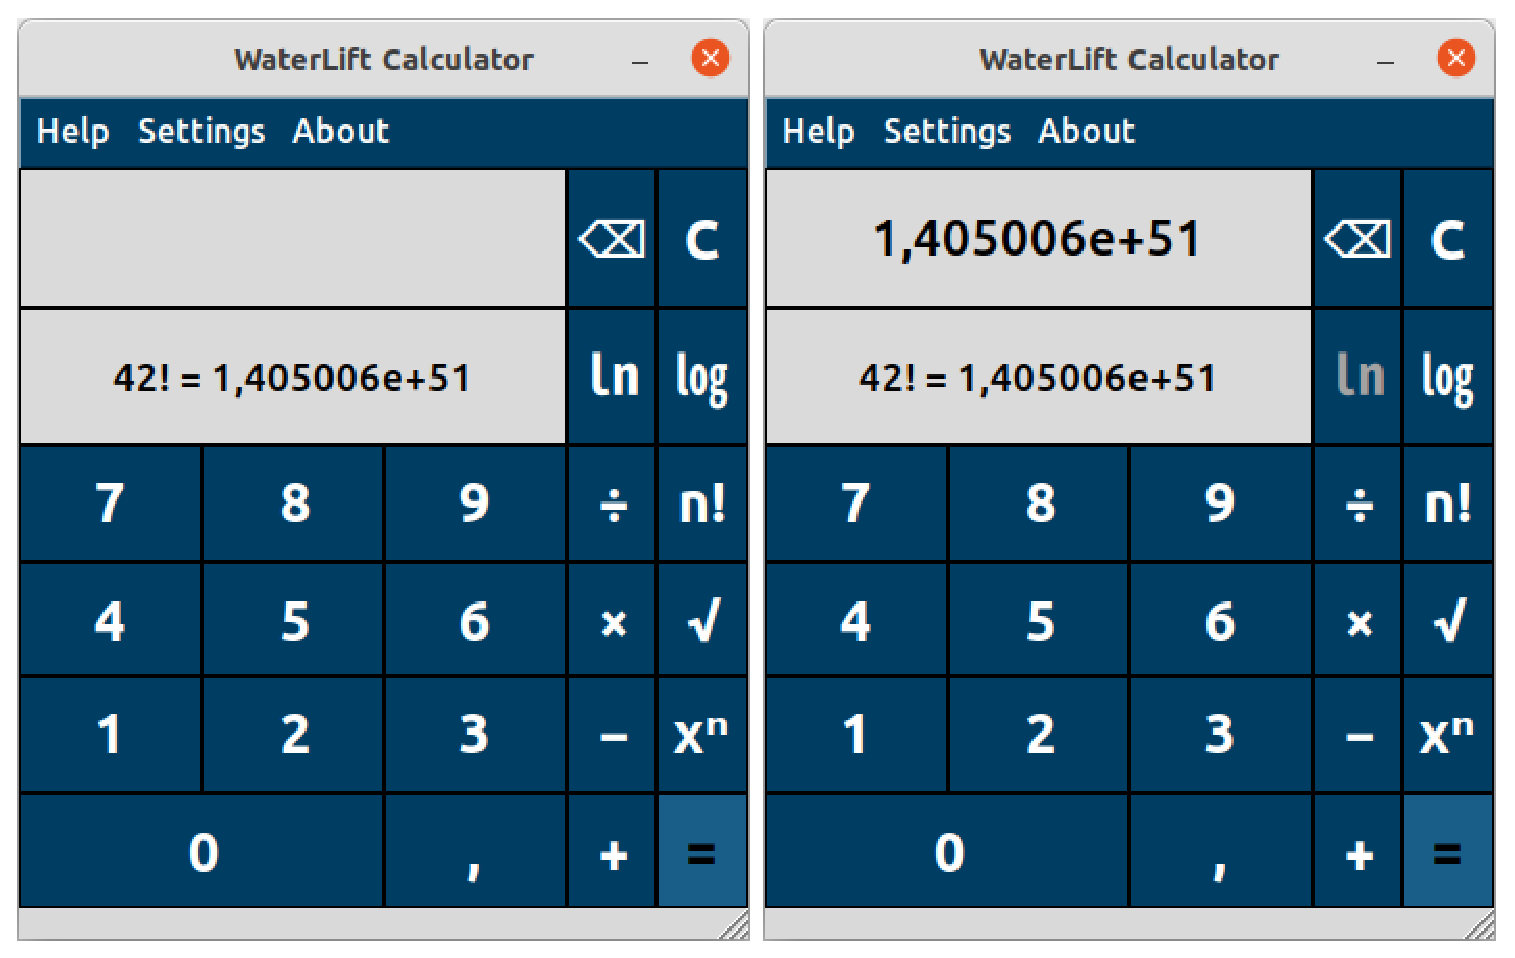
\includegraphics{continue_the_calculating01.eps}}
                    \caption{"Continue the calculating" feature}
                    \label{pic:continue_the_calculating01}
                \end{figure}
            \pagebreak
                \item or press the operation sign (except \keys{√}, \keys{log}, \keys{ln}) to put the result into the input field with it.
                \begin{figure}[h]
                    \centering
                    \scalebox{0.32}{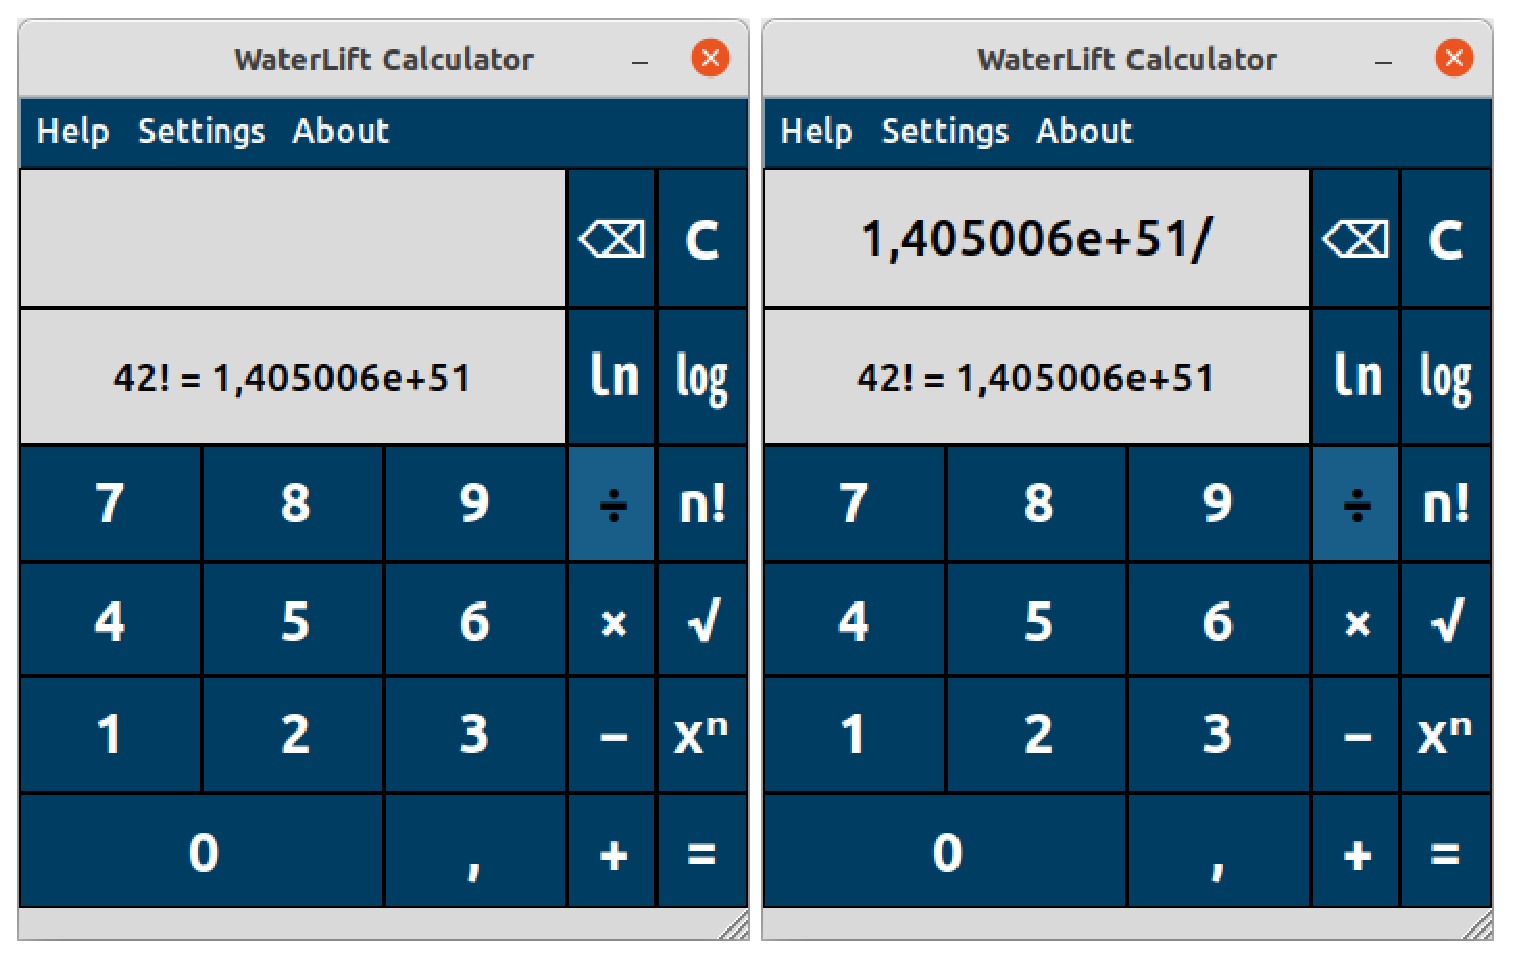
\includegraphics{continue_the_calculating02.eps}}
                    \caption{"Continue the calculating" feature}
                    \label{pic:continue_the_calculating02}
                \end{figure}
            \end{itemize}

        \subsubsection{"Change the operation sign"}
            When you put an operation sign into the input field, you can change it by pressing another.
            \begin{figure}[h]
                \centering
                \scalebox{0.32}{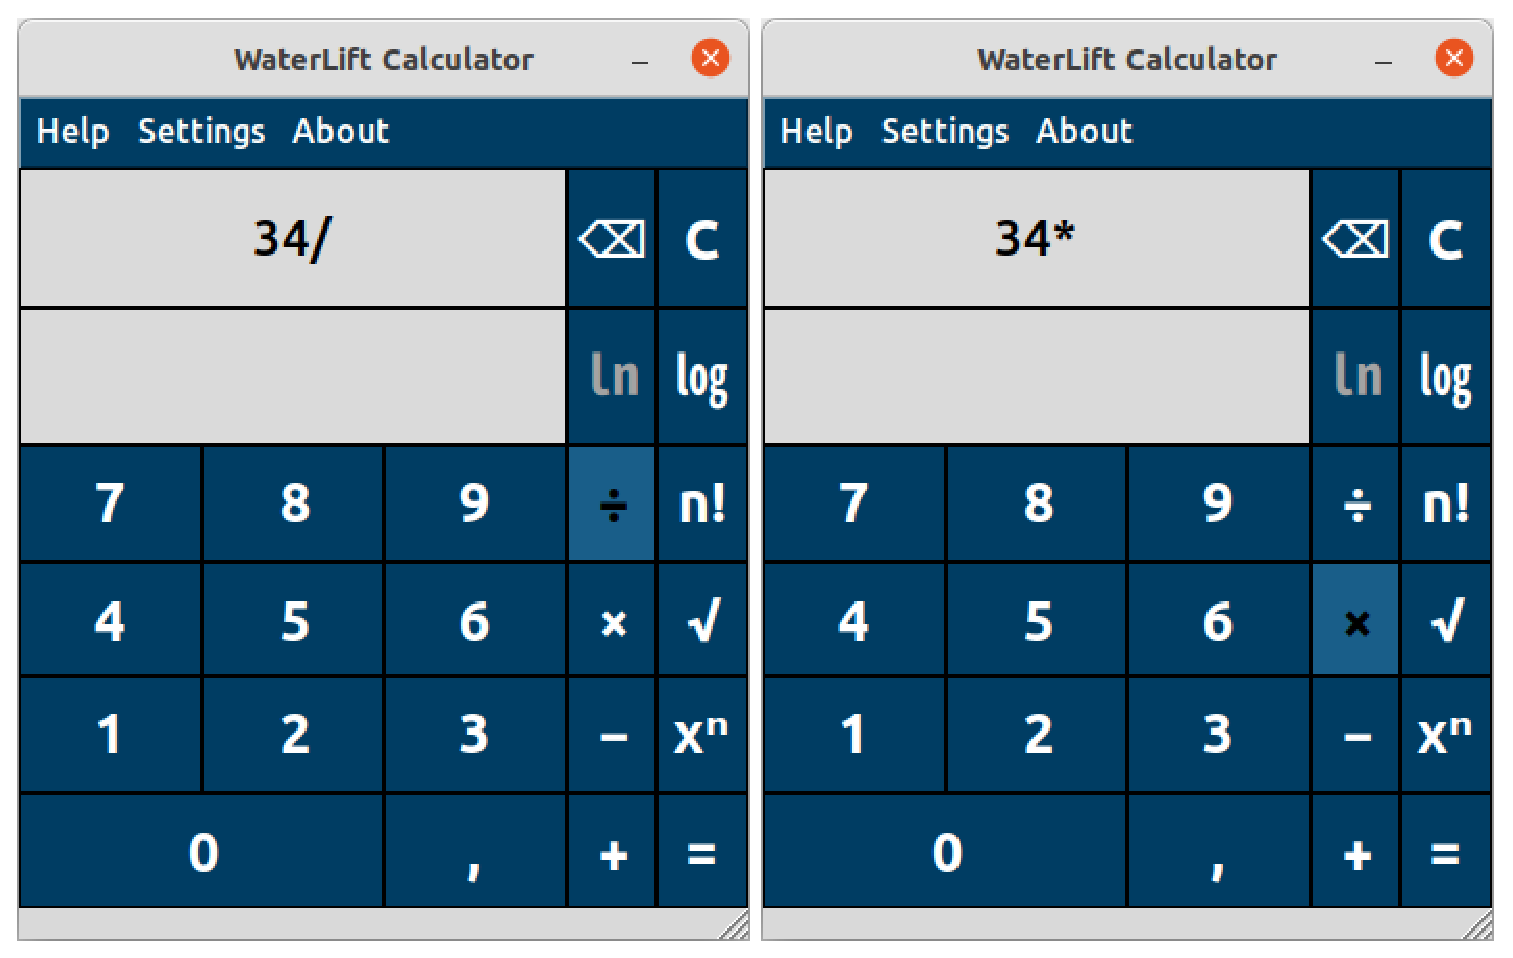
\includegraphics{change_the_operation_sign.eps}}
                \caption{"Change the operation sign" feature}
                \label{pic:change_the_operation_sign}
            \end{figure}

        \subsubsection{Window size control}
            You can change the window size by clicking the \keys{left mouse button} on the \emph{sizegrip} and moving the mouse.

        \subsubsection{Inactive buttons}
            The buttons become inactive if their using is impossible in the current expression.

        \subsubsection{Keyboard input support}
            We provide keyboard support for all input buttons. You can find Keyboard bindings table on the page \pageref{tab:Keyboard bindings}.

        \subsubsection{In-build user manual}
            You can always open a short version of this manual by clicking \keys{Help} or pressing the \keys{H} keyboard button.
            \begin{figure}[h]
                \centering
                \scalebox{0.24}{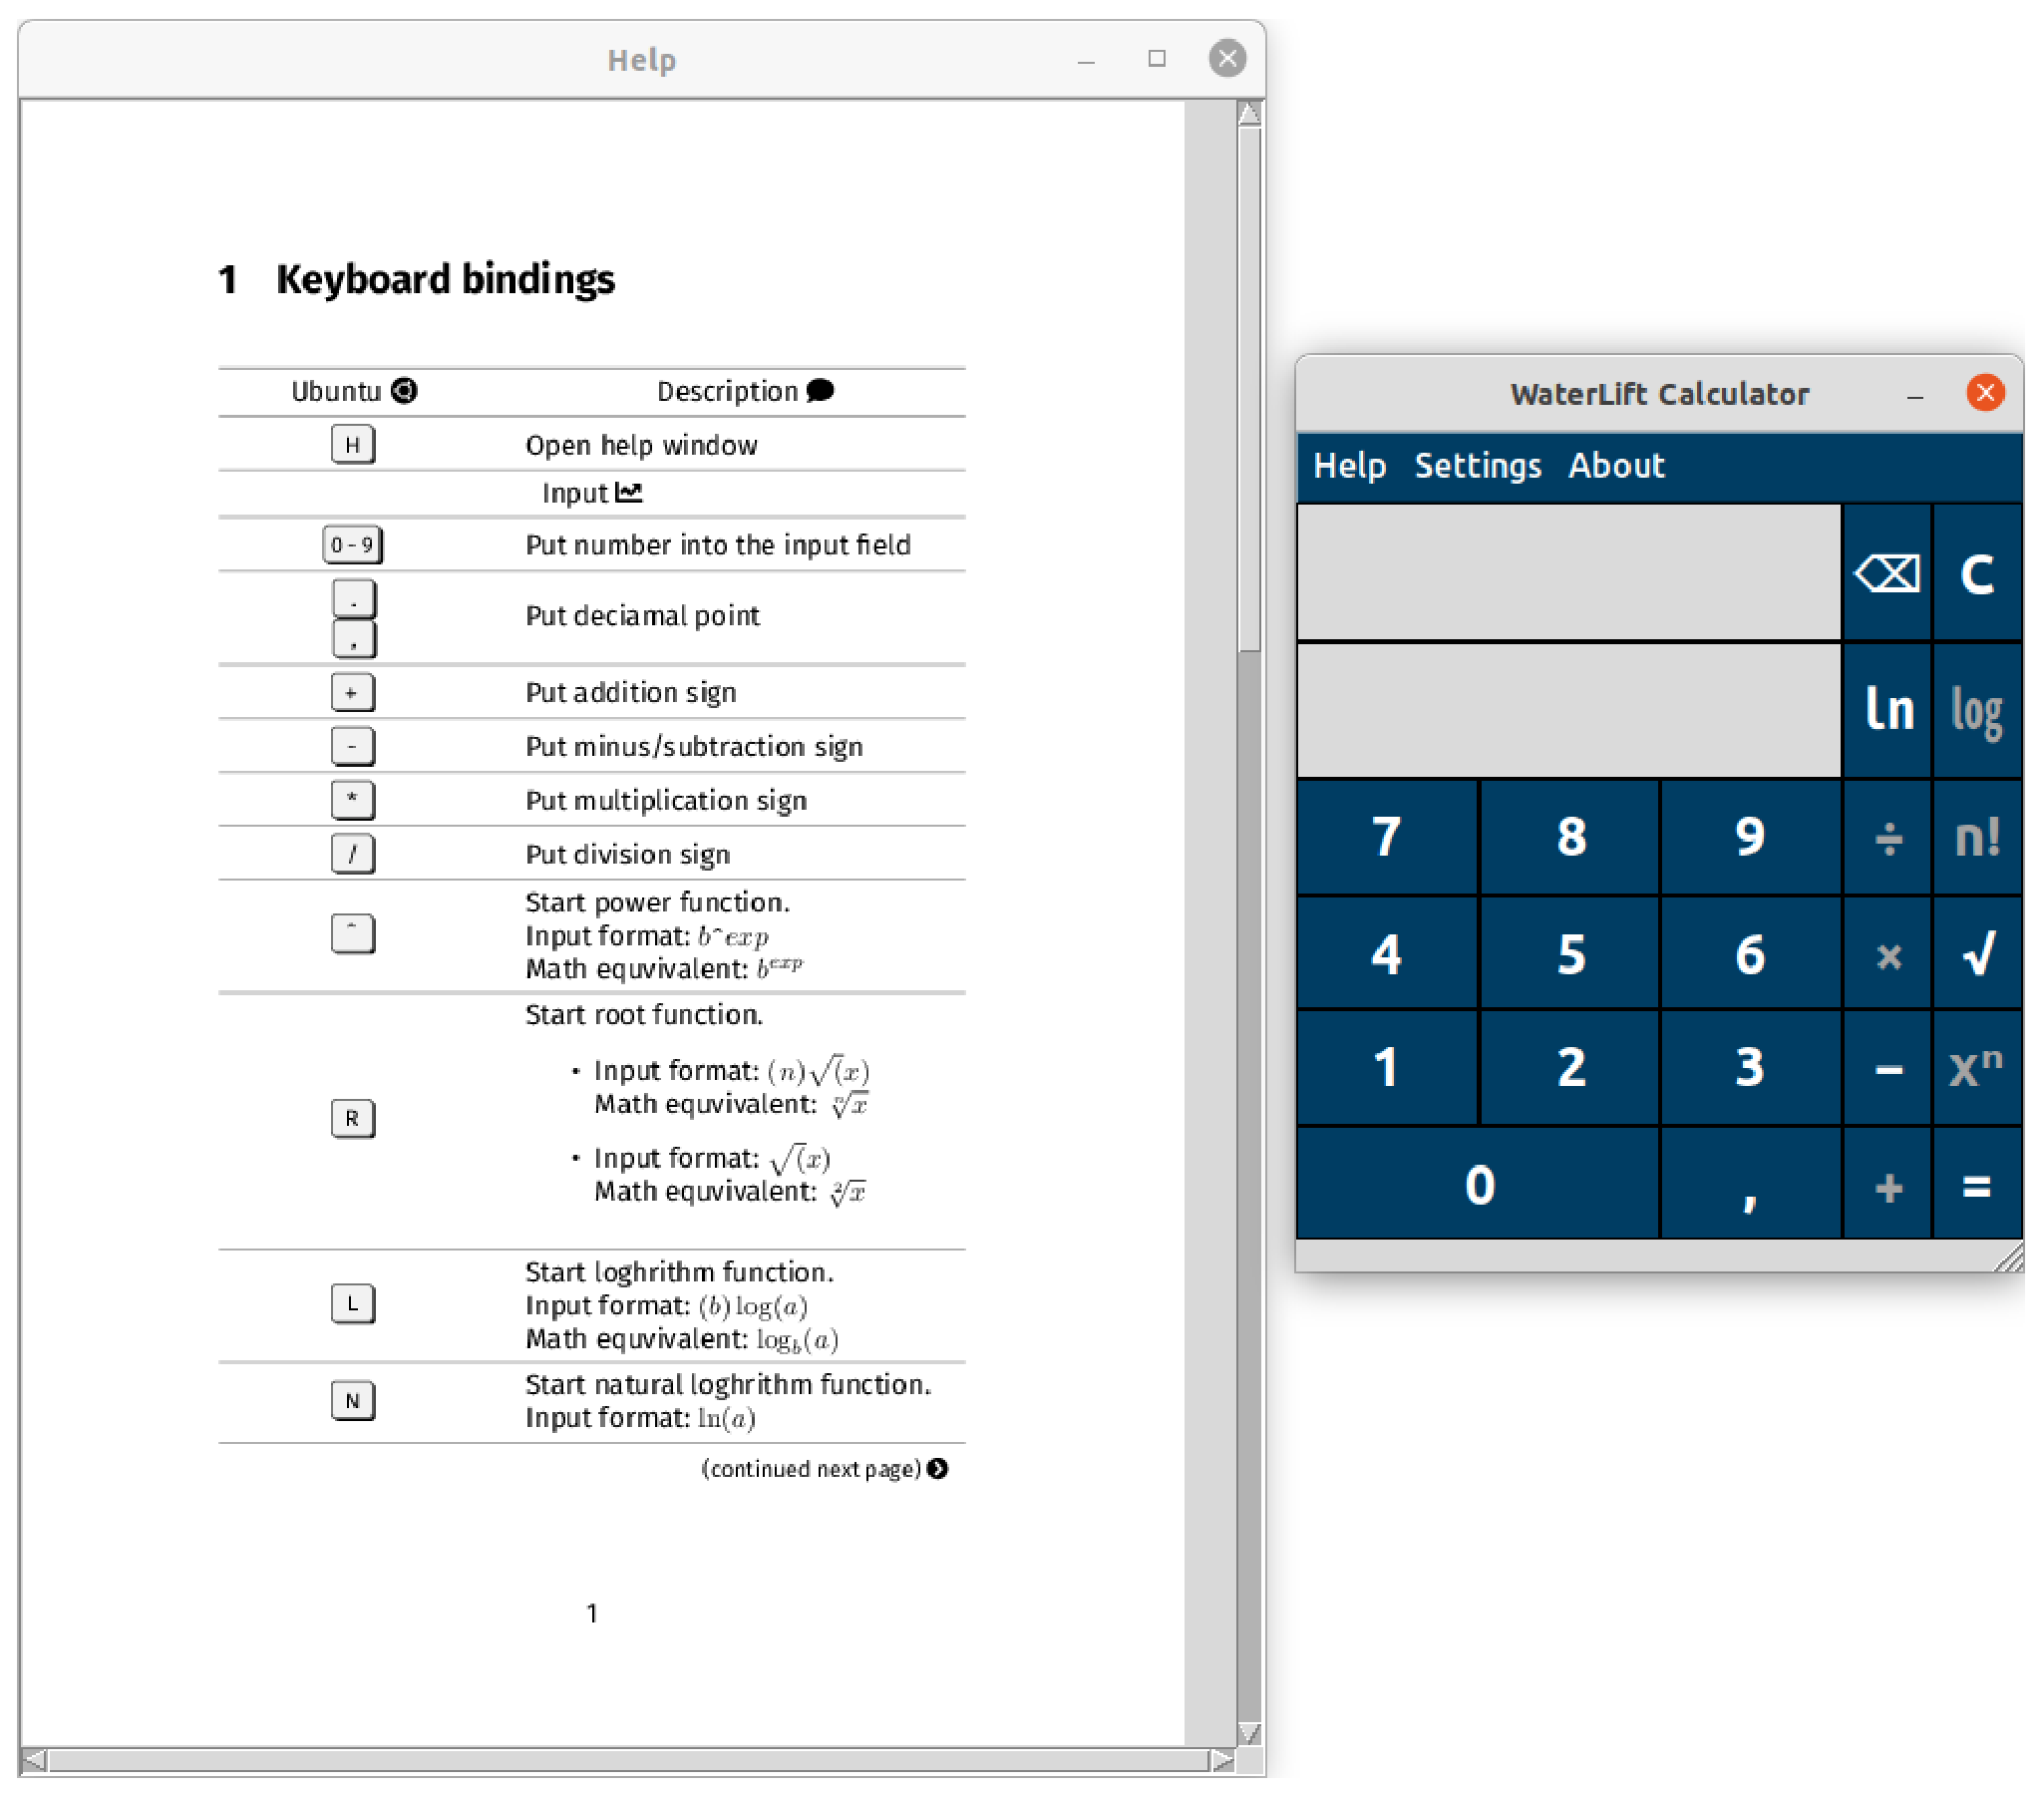
\includegraphics{help_window.eps}}
                \caption{In-build user manual}
                \label{pic:"in-build_use_manual"}
            \end{figure}

    \subsection{Operation limitations}
        \label{tab:operation_limits}
        \begin{xltabular}{\textwidth}{
            >{\setmenukeyswin}c @{\hspace{3em}}
            >{\renewcommand\cellalign{cl}}X}

            \toprule
            Operation \faCalculator & \multicolumn{1}{c}{Limitation \faTimesCircle}\\
            \midrule
            \endfirsthead

            \footnotesize \faChevronCircleLeft\ (from previous page)\\[1em]
            \toprule
            Operation \faCalculator & \multicolumn{1}{c}{Limitation \faTimesCircle}\\
            \midrule
            \endhead

            \\[-0.8em]
            \multicolumn{2}{r}{\footnotesize (continued next page) \faChevronCircleRight}
            \endfoot

            \bottomrule
            \endlastfoot

            \keys{\texttt{+}} & No limitation
            \\* \midrule

            \keys{-} & No limitation
            \\* \midrule

            \keys{*} & No limitation
            \\* \midrule

            \keys{$\div$} & $a\div b, b\neq 0$
            \\* \midrule

            \keys{\^{}} & $b^{exp}, exp\in \mathbb{N}$
            \\* \midrule

            \keys{$\sqrt{}$} &
            \begin{itemize}[leftmargin=*]
                \item  \vspace{-2em} $\sqrt[n]{x}, n \neq 0$
                \item  $\sqrt[n]{-x}, n \in \{2n+1|n \in \mathbb{Z}\}$\vspace{-1em}
            \end{itemize}
            \\* \midrule

            \keys{$\log$} & $\log_{b}{a}, b>0 \wedge b\neq 1, a>0$
            \\* \midrule

            \keys{$\ln$} & $\ln{a}, a>0$
            \\* \midrule

            \keys{!} & $n!, n \in \mathbb{N}$
            \\*
        \end{xltabular}

    \section{Keyboard bindings}
        \label{tab:Keyboard bindings}
        \begin{xltabular}{\textwidth}{
            >{\setmenukeyswin}c @{\hspace{3em}}
            >{\renewcommand\cellalign{cl}}X}

            \toprule
            Ubuntu \faUbuntu & \multicolumn{1}{c}{ Description \faComment}\\
            \midrule
            \endfirsthead

            \footnotesize \faChevronCircleLeft\ (from previous page)\\[1em]
            \toprule
            Ubuntu \faUbuntu & \multicolumn{1}{c}{ Description \faComment}\\
            \midrule
            \endhead

            \\[-0.8em]
            \multicolumn{2}{r}{\footnotesize (continued next page) \faChevronCircleRight}
            \endfoot

            \bottomrule
            \endlastfoot

            \keys{H} & Open help window
            \\* \midrule

           \multicolumn{2}{c}{\sffamily Input \faChartLine}
            \\* \midrule

            \keys{0 - 9} & Put the number into the input field
            \\* \midrule

            \makecell{%
            \keys{.}\\
            \keys{,}} & Put decimal point
            \\* \midrule

            \keys{\texttt{+}} & Put addition sign
            \\* \midrule

            \keys{-} & Put minus/subtraction sign
            \\* \midrule

            \keys{*} & Put multiplication sign
            \\* \midrule

            \keys{/} & Put division sign
            \\* \midrule

            \keys{\^{}} & Start power function. \newline Input format: $b\texttt{\^{}}exp$ \newline Math equivalent: $b^{exp}$
            \\* \midrule

            \keys{R} & Start root function.
            \begin{itemize}[leftmargin=*]
                \item  Input format: $n \sqrt x$ \newline Math equivalent: $\sqrt[n]{x}$
                \item  Input format: $\sqrt x$ \newline Math equivalent: $\sqrt[2]{x}$
            \end{itemize}
            \\* \midrule

            \keys{L} & Start logarithm function. \newline Input format: $(b)\log(a)$ \newline Math equivalent: $\log_b(a)$
            \\* \midrule

            \keys{N} & Start natural logarithm function. \newline Input format: $\ln(a)$
            \\* \midrule

            \keys{!} & Put factorial sign. \newline Input format: $n!$
            \\* \midrule

            \multicolumn{2}{c}{\sffamily Other \faKeyboard}
            \\* \midrule

            \makecell{%
            \keys{Enter}\\
            \keys{=}} & Evaluate the expression
            \\*
            \midrule

            \makecell{%
            \keys{Delete}\\
            \keys{BackSpace}} & Delete the last symbol from the input field. \newline If the input field is empty, clear the output field.
            \\*
            \midrule

            \keys{C} & Clear the input field. \newline If the input field is empty, clear the output field.
            \\* \midrule

            \keys{\esc} & Close the current window.\newline If was pressed on the main window, the application will be closed.
            \\*
        \end{xltabular}

\pagebreak

\section{Uninstallation}
    \subsection{Via the installer}
        Open the downloaded installer and click \keys{Remove} button\\
            \begin{figure}[h]
                \centering
                \scalebox{0.34}{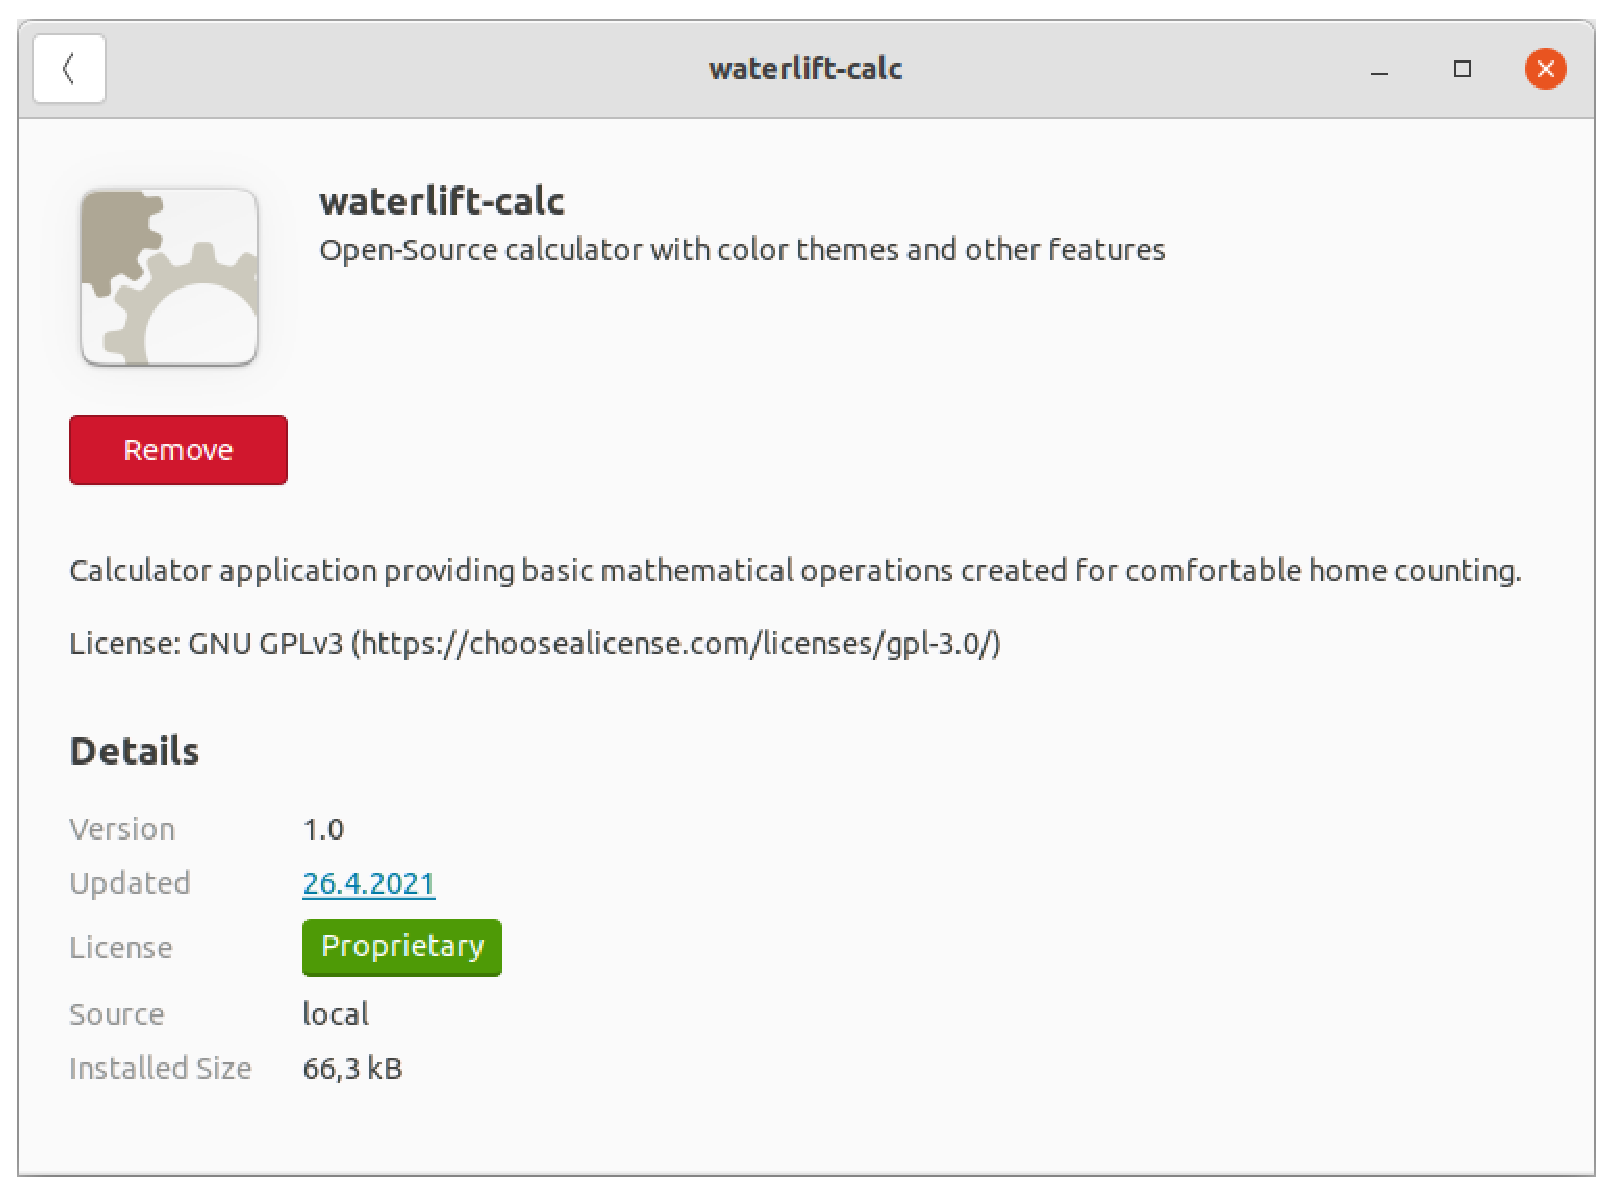
\includegraphics{uninstallation.eps}}
                \caption{Uninstallation window}
                \label{fig:uninstallation_window}
            \end{figure}
            
    \subsection{Via the CLI}
        \lstset{language=bash, frame=lines}
        \begin{lstlisting}
sudo dpkg -r waterlift-calc
        \end{lstlisting}
        
    \subsection{Manually}
    You can do all steps in any directory.
    \begin{enumerate}
        \item Give yourself superuser rights
            \lstset{language=bash, frame=lines}
            \begin{lstlisting}
sudo -s
            \end{lstlisting}
        \item Remove all app's files by the following commands:
            \begin{lstlisting}
rm -r /usr/bin/waterlift-calc

rm -r /usr/share/waterlift-calc/*

rmdir /usr/share/waterlift-calc

rm -r /usr/share/pixmaps/waterlift_calc_logo.png

rm -r /usr/share/applications/waterlift_calc.desktop
            \end{lstlisting}
    \end{enumerate}
        
You have successfully uninstalled the application.

\end{document}
